\documentclass[11pt,a4paper,fleqn]{article}
\usepackage[spanish,es-tabla]{babel}
\usepackage[utf8]{inputenc}
\usepackage{amsmath}
\usepackage{fp}
\usepackage{fancyhdr}
\usepackage{multirow}
\usepackage{caption}
\usepackage{xcolor}
\usepackage{ifthen}

\captionsetup{labelsep=period}
\usepackage{graphicx}
\graphicspath{ {Figuras/} }
\spanishdecimal{.}

%Datos
\newcommand\lVC{800}     %Claro de la viga
\newcommand\sVC{80}     %Separación de vigas
%Prpiedades geométricas
\newcommand\dW{79.4}     %Peralte del perfil
\newcommand\bfW{30}    %ancho del patín
\newcommand\tfW{2.2}    %espesor del patín
\newcommand\hrW{0}     %Distancia del borde superior de patin al concreto
\newcommand\tcW{10}       %Peralte de concreto
\newcommand\asW{240}  %Area de acero
%Propiedades de materiales
\newcommand\fy{2530}     %Resistencia del acero
\newcommand\fc{200}      %Resistencia del concreto


\begin{document}
\section{Ancho efectivo}

\begin{figure}[hbt]
  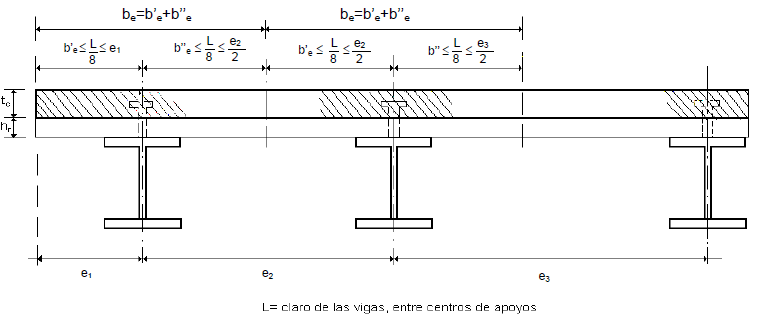
\includegraphics[scale=0.5]{Figuras/Be}
  \caption{Ancho efectivo de losa en sección compuesta}
  \label{fig:Be}
\end{figure}

El ancho efectivo de la losa de concreto, a cada lado de la viga de acero, se toma igual a la menor de las tres dimensiones siguientes (Figura \ref{fig:Be}):
\begin{enumerate}
	\item Un octavo del claro de la viga (L/8).
	\item La mitad de la distancia al eje de la viga ayacente.
\end {enumerate}

Considerando que tiene la misma distancia de los dos lados, se toma el doble de lo que se indico anteriormente siendo:

%Ancho efectivo
\FPeval{\lcuatro}{round(\lVC/4,2)}
\FPeval{\beVC}{round(min(\lcuatro,\sVC),2)}

\begin{enumerate}
	\item \begin{align*}
					b_e=\frac{\lVC}{4}=\lcuatro \text{ cm}
				\end{align*}
	\item \begin{align*}
					b_e=\sVC \text{ cm}
				\end{align*}
\end {enumerate}

Por lo que el ancho efectivo es \textcolor{blue}{\beVC \;cm}

\subsection{Resistencia a flexión}
el bloque de compresión del concreto se define como

\begin{equation}
	a=\frac{A_S f_y}{0.85f_{c}^{'}b_e}
\end{equation}

donde $a$ es el bloque de compresión del concreto, $A_S$ es el área de acero, $f_y$ es la resistencia del acero, $f_{c}^{'}$ es la resistencia del cocnreto y $b_e$ es el ancho efectivo.

Dependiendo de la distancia $a$ se pueden dar tres casos:

\begin{enumerate}
	\item  $a < t_c$ por lo que el ENP pasa por la losa.
	\item  $a > t_c$ y $C \geq T$ por lo que el ENP pasa por el patín.
	\item  $a > t_c$ y $C < T$ por lo que el ENP pasa por el alma.
\end {enumerate}

Donde $t_c$ es la capa de compresión del concreto, $C$ es la fuerza a compresión, $T$ es la fuerza a tensión y ENP es el eje neutro. 

Aplicando a los datos se tiene que el bloque de compresión es

%Bloque de compresión
\FPeval{\aVC}{round(\asW*\fy/(0.85*\fc*\beVC),2)}
\begin{align*}
	a=\frac{(\asW)(\fy)}{0.85(\fc)(\beVC)}=\aVC \text{ cm}
\end{align*}

\FPifgt \tcW \aVC  \FPeval{\pruebaVer}{1} \else \FPeval{\pruebaVer}{2} \fi %Evaluar si esta den losa o en viga
\ifthenelse{\pruebaVer=1}
	{%Eje neutro en losa
Como $(a=\aVC) < (t_c=\tcW)$, el eje neutro está en la losa por lo que el momento nominal se calcula con las ecuaciones siguientes

\begin{equation}
	M_n=A_sF_yd_1
\end{equation}

La distancia $d_t$ del centro de gravedad de la sección de acero al borde superior es:

\begin{equation}
		d_t=\frac{d}{2}
\end{equation}

El brazo del par de fuerzas interiores es:

\begin{equation}
		d_1=d_t+h_r+t_c-0.5a
\end{equation}

donde $h_r$ es la distancia entre el borde inferior de la losa y el superior de la viga

Por lo que al aplicarlo a los valores de este trabajo se tiene

\FPeval{\dtVC}{round(\dW/2,2)}
\begin{align*}
		d_t=\frac{\dW}{2}=\dtVC \text{ cm}
\end{align*}

\FPeval{\daVC}{round(\dtVC+\hrW+\tcW-\aVC/2,2)}
\begin{align*}
		d_1=\dtVC+\hrW+\tcW-0.5(\aVC)=\daVC \text{ cm}
\end{align*}

\FPeval{\mnVC}{round(\asW*\fy*\daVC/100000,2)}
\begin{align*}
		M_n=(\asW)(\fy)(\daVC)\times10^{-5}=\mnVC \text { t-m}
\end{align*}

Por lo que el momento resistente es

\FPeval{\mrVC}{round(\mnVC*0.85,2)}
\begin{align*}
		M_R=0.85(\mnVC)=\textcolor{blue}{\mrVC \text { t-m}}
\end{align*}
	}
	%else
	{
	Como $(a=\aVC) > (t_c=\tcW)$, el eje neutro está en la viga por lo que toda la losa trabaja a compresión siendo la fuerza del concreto 
\begin{equation}
		C_c=0.85f_{c}^{'}b_et_c
\end{equation}

Al estar el ENP sobre la viga, se pueden dar dos casos, uno cuando esta sobre el patín y otro sobre la viga por lo que se evalúan las fuerzas de compresión y tensión situando el ENP al borde inferior del patín por lo que
\begin{equation}
		C=C_c+A_{ps}F_y
\end{equation}

\begin{equation}
		T=(A_s-A_{ps})F_y
\end{equation}

Donde $C$ es la compresión sobre el ENP, $C_c$ es la compresión debia al concreto, $A_{ps}$ es el área del patín superior,$T$ es la tensión debajo del ENP y $A_{s}$ es el Area total del acero.
 
Por lo que
\FPeval{\ccVC}{round(0.85*\fc*\beVC*\tcW,2)}
\FPeval{\cVC}{round(\ccVC+(\bfW*\tfW*\fy),2)}
\FPeval{\tVC}{round((\asW-(\bfW*\tfW))*\fy,2)}
 
\begin{align*}
		&C_c=0.85(\fc)(\beVC)(\tcW)=&\ccVC \text{ kg} \\
		&C=\ccVC+(\bfW)(\tfW)(\fy)=&\cVC \text{ kg} \\
		&T=[\asW-(\bfW)(\tfW)]\fy=&\tVC \text{ kg} \\
\end{align*}
	
	\FPifgt \cVC \tVC  \FPeval{\pruebaVerB}{1} \else \FPeval{\pruebaVerB}{2} \fi %Evaluar si esta en patín
	\ifthenelse{\pruebaVerB=1}
	{
		Como la compresión es mayor a la tensión, el ENP esta en el patín por lo que el momento nominal se cálcula con
		
		\begin{equation}
			M_n=C_c d_2^{'} + C_a d_2^{''}
		\end{equation}
		 Para obtener las lineas de acción de las fuerzas se obtine la compresión del patín
		\begin{equation}
			C_a=\frac{A_s F_y-C_c}{2}
		\end{equation}
		
		y la profunidad de la zona comprimida del patín
		
		\begin{equation}
			t_{pc}=\frac{C_a}{b_f F_y}
		\end{equation}
		
		La distancia del centro de gravedad del área de acero en tensión al borde superior de la viga es
		
		\begin{equation}
			d_t=\frac{0.5A_sd-0.5b_f t_{pc}^2}{A_s-b_f t_{pc}}
		\end{equation}
		
		Las líneas de acción de las fuerzas a compresión y tensión son:
		\begin{equation}
			d_2^{'}=d_t+h_r+0.5t_c
		\end{equation}
		\begin{equation}
			d_2^{''}=d_t-0.5t_{tpc}
		\end{equation}
		
	Por lo que el momento nominal para este trabajo es:
	\FPeval{\caVC}{round((\asW*\fy-\ccVC)/2,2)} %Compresión del patín
	\FPeval{\tpcVC}{round(\caVC/(\bfW*\fy),2)} %Profunidad a compresión
	\FPeval{\dtVC}{round((0.5*\asW*\dW-0.5*\bfW*\tpcVC^2)/(\asW-\bfW*\tpcVC),2)} %distancia del acero al patin superior
	\FPeval{\dab}{round(\dtVC+\hrW+0.5*\tcW,2)} %d'2
	\FPeval{\daab}{round(\dtVC-0.5\tpcVC,2)} %d''2
	\FPeval{\mnVC}{round((\ccVC*\dab+\caVC*\daab)/100000,2)} %Momento nominal
		\begin{align*}
			&C_a=\frac{(\asW)(\fy)-\ccVC}{2}=&\caVC \text{ kg} \\
			&t_{pc}=\frac{\caVC}{(\bfW)(\fy)}=&\tpcVC \text{ cm} \\
			&d_t=\frac{0.5(\asW)-0.5(\bfW)(\tpcVC)^2}{\asW-(\bfW)(\tpcVC)}=&\dtVC \text{ cm} \\
			&d_2^{'}=\dtVC+\hrW+0.5(\tcW)=&\dab \text{ cm} \\
			&d_2^{''}=\dtVC-0.5(\tpcVC)=&\daab \text{ cm} \\
			&M_n=[(\ccVC)(\dab) + (\caVC)(\daab)]\times 10^{-5}=&\mnVC \text{ ton-m}
		\end{align*}
		Por lo que el momento resistente es

		\FPeval{\mrVC}{round(\mnVC*0.85,2)}
		\begin{align*}
				M_R=0.85(\mnVC)=\textcolor{blue}{\mrVC \text { t-m}}
		\end{align*}
	}
	%else
	{
		Como la compresión es menor a la tensión, el ENP esta en el alma por lo que el momento nominal se cálcula con
		\begin{equation}
			M_n=C_c d_2^{'} + C_a d_2^{''}
		\end{equation}
		 Para obtener las lineas de acción de las fuerzas se obtine la compresión del patín
		\begin{equation}
			C_a=\frac{A_s F_y-C_c}{2}
		\end{equation}
		Profunidad del alma a compresión
		
	}%fin if
}%fin if
\end{document}